%\graphicspath{{~/Pictures/Screenshots/}} % path to graphics
\graphicspath{{./img/}} % path to graphics

\chapter*{Цель практической работы}
\addcontentsline{toc}{chapter}{Цель практической работы}
Создать чат-бота для соц. сети Telegram. Разобраться и научиться работать
с Telegram API. Ознакомиться с формулированием функциональных
требований к проекту в виде User Story. Разработать интерфейс бота.
Выбрать систему контролей версий и научиться с ней работать.

\chapter{Система контроля версий и оформление кода}
\section{Функциональные требования}
User Story --- это короткая формулировка намерения, описывающая что-то,
что система должна делать для пользователя.\par
Текст самой user story должен объяснять роль/действия юзера в системе,
его потребность и профит, который юзер получит после того как история
случится. К примеру: \textbf{Как, <роль/персонаж юзера>, я <что-то хочу
получить>, <с такой-то целью>}.

User Story, оформленные в виде карточек, предоставленны в
таблицах~\ref{table:user_story:info:stud}\,-\,\ref{table:user_story:info:teacher}.

\begin{table}[h!tp]
	\centering
	\caption{\leftline{Карточка User Story}}
	\label{table:user_story:info:stud}
	\begin{tabular}{|l|l|l|}
		\hline \multicolumn{2}{|l|}{Заголовок} & Информация о очереди\\ \hline
		Заказчик (actor) & Как & Студент \\ \hline
		Примечание & Я хочу & Отслеживать порядок очереди\\ \hline
		Цель & Чтобы & Знать заранее когда сдаю я\\ \hline
	\end{tabular}
\end{table}
\begin{table}[h!tp]
	\centering
	\caption{\leftline{Карточка User Story}}
	\label{table:user_story:notify}
	\begin{tabular}{|l|l|l|}
		\hline \multicolumn{2}{|l|}{Заголовок} & Уведомления\\ \hline
		Заказчик (actor) & Как & Студент \\ \hline
		Примечание & Я хочу & Получить уведомление\\ \hline
		Цель & Чтобы & Не пропустить свою очередь сдавать работу\\ \hline
	\end{tabular}
\end{table}
\begin{table}[h!tp]
	\centering
	\caption{\leftline{Карточка User Story}}
	\label{table:user_story:exit}
	\begin{tabular}{|l|l|l|}
		\hline \multicolumn{2}{|l|}{Заголовок} & Выход из очереди\\ \hline
		Заказчик (actor) & Как & Студент \\ \hline
		Примечание & Я хочу & Выйти из очереди после сдачи\\ \hline
		Цель & Чтобы & Очередь продвигалась\\ \hline
	\end{tabular}
\end{table}
\begin{table}[h!tp]
	\centering
	\caption{\leftline{Карточка User Story}}
	\label{table:user_story:entrance}
	\begin{tabular}{|l|l|l|}
		\hline \multicolumn{2}{|l|}{Заголовок} & Вступление в очередь\\ \hline
		Заказчик (actor) & Как & Студент \\ \hline
		Примечание & Я хочу & Вступить в очередь\\ \hline
		Цель & Чтобы & Получить уведомление об очереди\\ \hline
	\end{tabular}
\end{table}
\begin{table}[h!tp]
	\centering
	\caption{\leftline{Карточка User Story}}
	\label{table:user_story:create}
	\begin{tabular}{|l|l|l|}
		\hline \multicolumn{2}{|l|}{Заголовок} & Создание очереди\\ \hline
		Заказчик (actor) & Как & Староста \\ \hline
		Примечание & Я хочу & Иметь возможность создавать очередь\\ \hline
		Цель & Чтобы & Мои одногруппники могли в нее встать\\ \hline
	\end{tabular}
\end{table}
\begin{table}[h!tp]
	\centering
	\caption{\leftline{Карточка User Story}}
	\label{table:user_story:info:elder}
	\begin{tabular}{|l|l|l|}
		\hline \multicolumn{2}{|l|}{Заголовок} & Информация о очереди\\ \hline
		Заказчик (actor) & Как & Староста \\ \hline
		Примечание & Я хочу & Знать кто сдавал работы\\ \hline
		Цель & Чтобы & Исправить возможную ошибку в журнале\\ \hline
	\end{tabular}
\end{table}
\begin{table}[h!tp]
	\centering
	\caption{\leftline{Карточка User Story}}
	\label{table:user_story:info:teacher}
	\begin{tabular}{|l|l|l|}
		\hline \multicolumn{2}{|l|}{Заголовок} & Информация о очереди\\ \hline
		Заказчик (actor) & Как & Преподаватель \\ \hline
		Примечание & Я хочу & Видеть сколько осталось студентов\\ \hline
		Цель & Чтобы & Распланировать время\\ \hline
	\end{tabular}
\end{table}

\section{Интерфейс разрабатываемого продукта}
Так как в данном проект разрабатывался telegram-бот, интерфейс и дизайн,
по большей степени, зависит от приложения telegram. От прогрммиста
зависит только интуитивная понятность диалога пользователя с ботом.
Так что, внешне, интерфейс приложения не будет существенно отличаться от
существующий telegram-ботов. Пример, на основе аналога, показан
на рисунке~\ref{fig:interface:analog}.
\begin{figure}[h!tp]
	\centering
	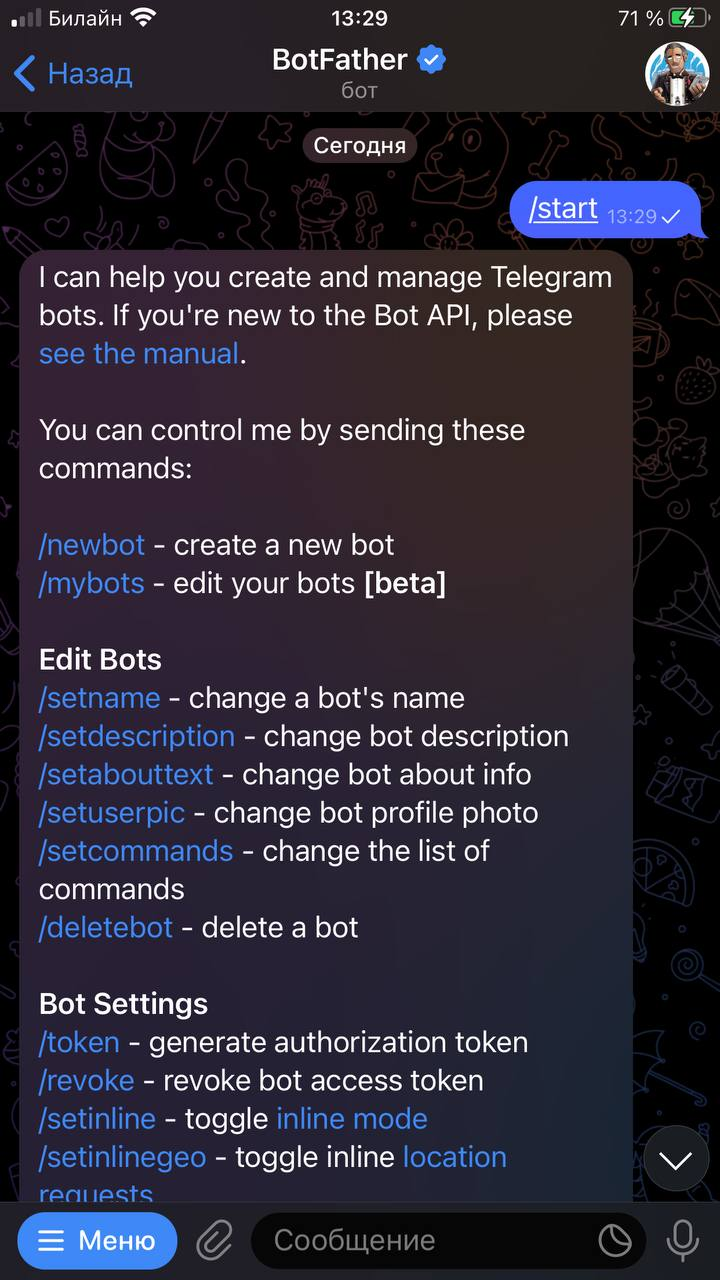
\includegraphics[width=0.55\textwidth]{TelegramBotInterface}
	\caption{Пример интерфейса}
	\label{fig:interface:analog}
\end{figure}

